%!TeX spellcheck = fr-FR
\documentclass[10pt,fleqn]{article} % Default font size and left-justified equations
\usepackage[%
    pdftitle={La chain d'énergie},
    pdfauthor={Geoffrey Vaquette}]{hyperref}

\usepackage{import}
\usepackage{subcaption}
\subimport{../../../../style/}{preambule.tex}
%\fichetrue
\fichefalse
\proftrue
%\proffalse
%\tdtrue
\tdfalse
\courstrue
%\coursfalse
\subimport{../../../../style/}{new_style}
\subimport{../../../../style/}{macros_SII}
\subimport{../../../../style/}{preambule_trou.tex}

\usepackage{siunitx}
% -------------------------------------
% Déclaration des titres
% -------------------------------------

\def\discipline{Enseignement \\Technologique \\ Transversal}
\def\xxtete{Enseignement Technologique Transversal}

\def\classe{1 STI2D}
\def\xxnumpartie{Seq 3}
\def\xxpartie{La chaîne d'énergie}

\def\xxnumchapitre{Séance 3}
\def\xxchapitre{\hspace{.12cm} Synthèse}

\def\xxposongletx{2}
\def\xxposonglettext{1.45}
\def\xxposonglety{23}
\def\xxonglet{Seq. 3 -- Se. 3}

\def\xxactivite{Cours}
\def\xxauteur{\textsl{Geoffrey Vaquette}}

\def\xxcompetences{%
\textsl{%
\textbf{Prérequis :}
\begin{itemize}[label=\ding{112},font=\color{ocre}]
\item Analyse fonctionnelle de la chaîne d'énergie
\end{itemize}
\textbf{Savoirs et compétences :}
\begin{itemize}[label=\ding{112},font=\color{ocre}]
\item CO2.1	Identifier les flux et la forme de l'énergie, caractériser ses transformations et/ou modulations et estimer l'efficacité globale d'un système.
\end{itemize}
%
}}

\def\xxfigures{
\begin{center}
% 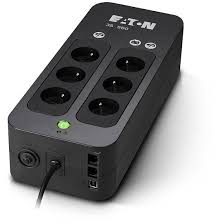
\includegraphics[width=2cm]{images/onduleur} \\
% 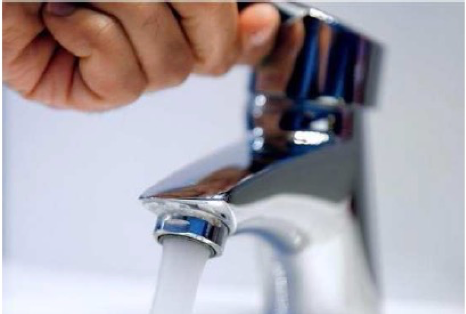
\includegraphics[width=2cm]{images/robinet} \\
%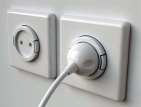
\includegraphics[width=2cm]{images/prise.png} \\
\end{center}
}%figues de la page de garde
\def\xxpied{%
La chaîne d'énergie \xxactivite%
}

%---------------------------------------------------------------------------

\renewcommand{\RemplirTrou}{false}
\begin{document}
\chapterimage{images/chaine}
\subimport{../../../../style/}{new_pagegarde}

\begin{figure}[h]
  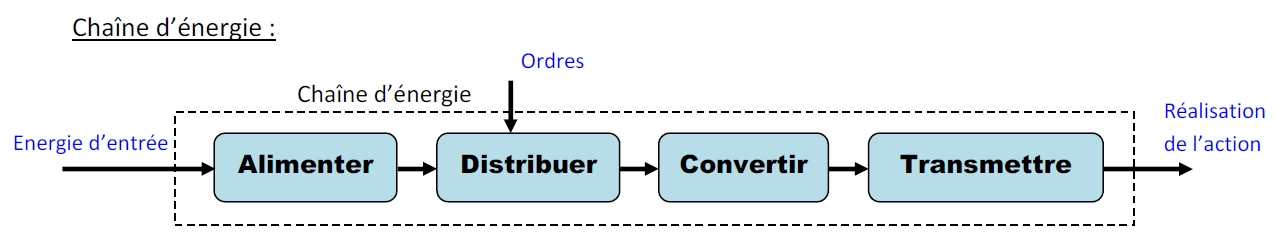
\includegraphics[width=\textwidth]{images/chaine}
  \caption{Les quatre blocs de la chaine d'énergie}
  \label{fig:chaine}
\end{figure}

Dans cette séquence, nous avons abordé les quatre blocs de la chaine d'énergie. Pour chacun d'eux, nous avons défini sa fonction et donné des exemples de composant permettant de remplir cette fonction. Durant cette dernière séance, nous allons passer rapidement en revue les principales notions que nous avons abordées.

\section{Le bloc Alimenter}
\begin{defi}
    Les éléments du bloc \textbf{Alimenter/Stocker} ont pour fonction de \trou{fournir l'énergie au système}. Cette énergie peut provenir \trou{de l'extérieur du système (Réseau électrique par exemple)} ou être \trou{stockée au sein du système (Batterie électrique par exemple)}.
\end{defi}

\subsection{Stockage et circulation de charges électriques}
On peut stocker de l'énergie dans des batteries, des piles.

\begin{aretenir}
  Un courant électrique, c'est un déplacement de \trou{charges électriques $q$}. L'intensité représente le \trou{débit de charges électriques} se déplaçant dans un conducteur électrique.

  \fbox{\large$q = I\times t$} \hfill \fbox{\SI{1}{A} = \SI{1}{C/s}}
\end{aretenir}

Puisqu'un courant électrique est un déplacement de charges électriques, il paraît naturel de caractériser le stockage d'énergie électrique par le nombre de charges que ce stockage permettra de fournir.

\begin{aretenir}
  Puisque $q = I\times t $, un courant multiplié par un temps représente un nombre de charge (les \si{Ah} représente donc un nombre de charges).
  \hfill\fbox{\large$\SI{1}{Ah} = \SI{3600}{C}\times t$}\hfill
\end{aretenir}

Les charges électriques se déplacent sous l'effet d'une \trou{différence de potentiel} (ou tension).

\begin{aretenir}
  La puissance électrique est le produit de la tension et du courant circulant dans un dipôle.
  \hfill\fbox{\large$P = U\times I $}\hfill
\end{aretenir}

\paragraph{Règles d'associations de batteries}
\begin{aretenir}
  Lorsque deux batteries sont branchées en \textbf{série}, leurs tensions \trou{s'ajoutent} et leurs capacité \trou{sont identiques}.
\end{aretenir}

\begin{aretenir}
  Lorsque deux batteries sont branchées en \textbf{parallèle}, leurs tensions \trou{sont identiques} et leurs capacité \trou{s'ajoutent}.
\end{aretenir}

\section{Le bloc distribuer}
\begin{definition}
  L'énergie fournie par le bloc \textit{alimenter} est \trou{distribuée} par le bloc \textit{Distribuer}.
  Cela signifie que l'énergie est \trou{adaptée et dirigée} vers les différents organes du système.
\end{definition}

\subsection{Les relais et les contacteurs}
\begin{aretenir}
  Les relais et les contacteurs sont des \trou{interrupteurs commandés} qui fonctionne grâce à une \trou{bobine} qui se comporte comme un aimant.
\end{aretenir}

\subsection{Les transistors}
\begin{figure}
  \centering
  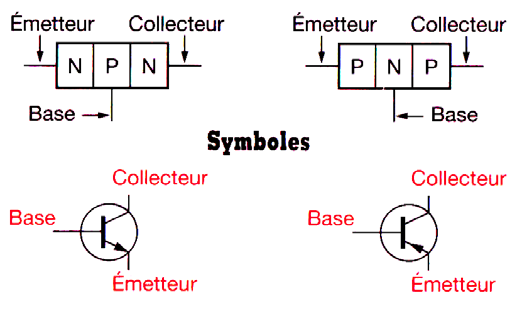
\includegraphics[width=.5\textwidth]{images/schema_transistor}
  \caption{Transistors bipolaires }
  \label{}
\end{figure}
\begin{aretenir}
  Lorsqu'ils sont utilisés en \textbf{saturation}, les transistors se comportent comme des interrupteurs commandés.
\end{aretenir}

\subsection{Commander un Courant à Continu : Le pont en H}

\begin{figure}[h]
  \centering
  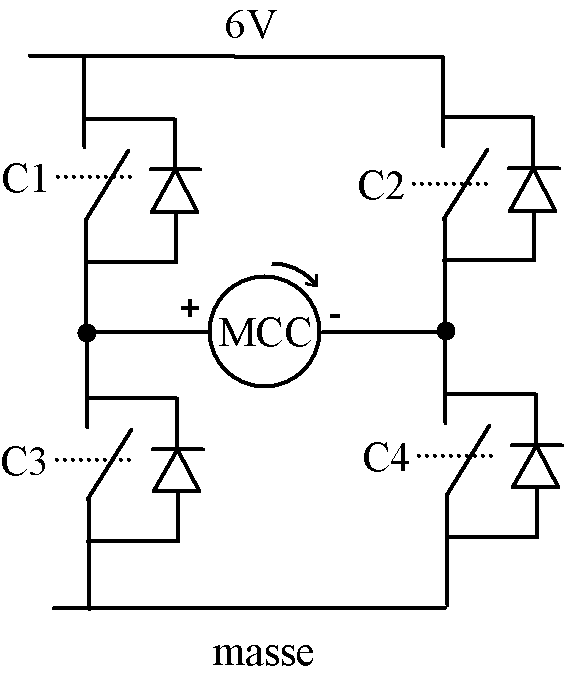
\includegraphics[height=.35\textheight]{images/pontH}
  \caption{Pont en H}
  \label{pont en H}
\end{figure}

\begin{itemize}
  \item Lorsque le moteur est alimenté normalement, c’est à dire lorsque le 6V est sur le + et la masse (0V) sur le -, le moteur tourne dans le sens indiqué.
  \item Si on inverse, c’est à dire si la masse est sur le + et le 6V sur le -, le moteur tourne dans l’autre sens.
\end{itemize}

\begin{exemple}
  Pour faire tourner le moteur dans le sens indiquer, il faut fermer \trou{C1} et \trou{C4}.
\end{exemple}

\begin{exemple}
  Pour faire tourner le moteur dans le sens inverse, il faut fermer \trou{C2} et \trou{C3}.
\end{exemple}

\section{Le bloc convertir}
  \begin{definition}
    Les composants réalisant la conversion d’énergie sont appelés « actionneurs » : ils permettent de convertir l'énergie reçue en travail utile pour exécuter les tâches du système.
  \end{definition}

\subsection{Les moteurs}
\begin{aretenir}
  Les moteurs sont constitués d'un \trou{stator} qui est fixe et d'un \trou{rotor} qui tourne.
\end{aretenir}

\subsubsection{Les moteurs à courant continu}
\begin{aretenir}
  La vitesse de rotation \trou{est proportionnelle à } la tension d'alimentation du moteur.
  $$\Omega = K\times U$$
  avec $K$ la constante du moteur à courant continu.
\end{aretenir}

\section{Le bloc transmettre}


\subsection{Les engrenages}




\begin{figure}[h]
  \centering
  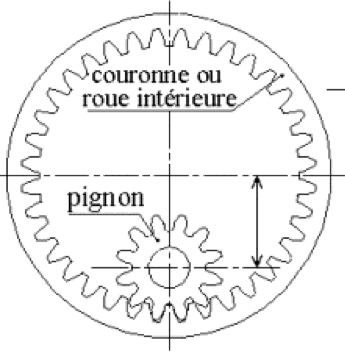
\includegraphics[width=.3\textwidth]{images/engre_interieur}
  \hfill
  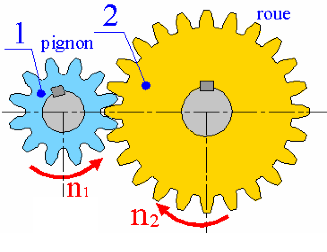
\includegraphics[width=.4\textwidth]{images/engrenage_2_droit}
  \caption{Engrenage à contact intérieur et exterieur}
  \label{}
\end{figure}

\begin{definition}
  Le rapport $r$, aussi appelé \textit{raison de l'engrenage} est égal à $$r = \frac{Z_{\text{menante}}}{Z_{\text{menée}}} = \frac{\omega_s}{\omega_e}$$

  Avec $Z$ le nombre de dents des roues menante et menée et $\omega_s$ et $\omega_e$ les vitesse d'entrée et de sortie, respectivement.
\end{definition}

\begin{description}
  \item [Si $r<1$] \trou{$r$ est un rapport de réduction car la vitesse de sortie est plus faible que la vitesse d'entrée}
  \item [Si $r>1$] \trou{$r$ est un rapport de transmission. La vitesse de sortie est plus forte que la vitesse d'entrée. }
  \item [Si $r=1$] \trou{La vitesse en entrée est égale à la vitesse en sortie}
\end{description}

\begin{aretenir}
  $$r_{eq} = r_1 \times r_2 \times \dots \times r_n $$
  donc
  $$\omega_s = (-1)^n r_{eq} \omega_e$$
  Dans le cas de contacts exterieurs, le nombre de contacts exterieurs conditionne le sens de rotation en sortie.
\begin{description}
  \item [Si n est pair] \trou{Le sens de rotation en sortie est le même que celui en entrée}
  \item [Si n est impair] \trou{Le sens de rotation en sortie est inversé par rapport à celui de l'entrée}
\end{description}
\end{aretenir}

\end{document}
